\subsection{Reflection of our process}

Overall, we exceeded all of our expectations this year. We did an excellent job of identifying reusable code from XSquare, and modifying/augmenting it for our own purposes. This allowed us to get out a high-quality bot much quicker than previous years.

\medskip

From there, we did a good job of identifying key, game-specific tasks to implement, such as capturing towers, basic combat, and opening logic. This allowed our team to achieve good results quickly, as these tasks had the highest reward for the lowest effort.

\medskip

Finally, we were able to make consistent improvements to our bot by identifying inefficiencies in resource management and idle time. These efforts were all it took for our team to make the leap to being a top-level team.

\medskip

However, there were certainly areas where we could improve. Justin spent a lot of time re-doing XSquare code such as pathfinding when realistically, he couldn't really improve it and ended up wasting a lot of time. Andrew spent a lot of time on the SURVIVE behavior of bots, which was not an efficient use of his time since the SURVIVE behavior never really impacted the result of any matches. It was Matt's first year, so he was climbing the learning curve while also being busy with class.

\medskip

Additionally, the way we ended up dealing with goal objectives was messy. Each robot was able to keep track of multiple different goal objectives, however, we didn't define a formal framework for how to resolve having multiple different goal objectives. As a result, our goal resolution was a bunch of unorganized if-statements that was difficult to modify/debug. We could've benefited greatly from a formal goal resolution framework, so we will give one in the next section.

\medskip

Finally, we did not pay that much attention to other teams' strategies. Copying other teams' strategies is a Battlecode staple because it allows you to easily identify improvements for your own bot that other teams have conveniently tested for you. Our team neglecting this strategy resulted in a unique bot. However, it also resulted in our bot lacking obvious features such as ignoring refills, having a good build order, and having soldiers seek out enemy towers to kill.

\subsection{Reflection on the game}

The game this year was probably the best game we've taken part in. The 2025 game did a great job removing all of the game elements that made the last 2/3 years micro-heavy games while also adding new elements that made decision-making interesting. 

\medskip

Opening theory was interesting since choosing between double soldier openings, rushing, mopper openings, or even SRP/splasher openings was a non-obvious choice. 

\medskip

Paint management was a very interesting task since you had to balance normal pathfinding, staying on allied paint, and choosing when to paint tiles where no option was the obvious choice.

\medskip

Build order being an essential part of the gameplan was back from 2021, since you always had the option to build every robot type and every tower type. Each team had to tackle difficult questions such as ``when do we start building splashers?'' or ``when are defense towers worth it?''

\medskip

SRPs were a great addition, since they gave access to an NP problem (a packing problem) that could be solved at any time for a small economic gain. However, since it was nearly always more worth it to capture more towers, it provided an interesting choice: explore for ruins, or build SRPs. Additionally, since finding the optimal SRP placement is an NP problem, it meant that every team could have slightly different approximation algorithms for SRP placement.

\medskip

Overall, Teh Devs did a fantastic job releasing patches. They did a great job of nerfing overtuned strategies such as SRP spam or rushing while not making those strategies useless with the nerfs. However, we have some gripes with how they treated defense towers. 

\medskip

Historically, static defense in Battlecode was never a meta-relevant strategy. In 2022, watchtowers were weak since they were a large investment, which was a death sentence in that year's game since cheap units could snowball very quickly. However, the 2025 game was the perfect opportunity for static defense. Robots not being able to engage in direct combat with each other meant that offense and defense could be separate entities, i.e.: a good offense wouldn't just automatically double as a good defense, which would've given static defense a unique role. Additionally, map control was crucial to the game, so static defense having higher power in exchange for not being able to move would've been an appealing trade-off.

\medskip

However, Teh Devs caved to early complaints about defense tower being too strong before sprint 1 even happened. The defense tower nerfs came too early in our opinion, since they never saw tournament results, and Teh Devs didn't have faith in the inherent weaknesses of static defense. In the end, defense towers just turned into slightly different money towers.

\medskip

Static defense is a fascinating game aspect that we believe still hasn't been fully explored by Teh Devs. Static defense's polarizing strength is offset by a resource investment and the opportunity cost of investing in resource-economy instead. In RTS games, the counter to static defense is to disengage and gain an economic advantage since the opponent put a large investment in static defense. We believe this would add an extra dimension to any meta, since every Battlecode meta usually devolves into ``always attack.''

\medskip

Overall, Teh Devs made massive improvements this year. They upgraded to a newer Java version, they added Python compatibility, they updated the client, and they made the best game in years. They deserve all the praise, and we are optimistic they can keep the good momentum into next year.

\subsection{Advice}

We have learned a lot through our years of Battlecode. This includes resources that we've compiled from across many teams' experiences. If you are reading this, it's likely you aren't actively competing. Here's some advice you can either actively follow outside of competition, or keep in mind for the next upcoming competition.

\begin{enumerate}
  \item \textbf{Spend time preparing} - Before the competition starts, read Postmortems, look at code from other teams, and make a general plan for how you want to break up work amongst your team. You can even create a structure for your code ahead of time. For us, using a \verb|Robot| base class and different utility classes (\verb|MapData|, \verb|Communication|, etc.) seems to have worked the best. Additionally, there are aspects of Battlecode that remain constant through nearly every year. They are as follows.
  \begin{itemize}
      \item \textbf{The Map} - The Battlecode map is (nearly) always a coordinate-grid of size between 20x20 and 60x60 inclusive. For fairness, the map is always symmetrical either by rotation or reflection. Essentially all top teams have some sort of map data structure in every bot that stores all known information about the map. Being able to identify which of the 3 symmetries (reflection over x-axis, reflection over y-axis, and rotation) the map contains, and extrapolating known information with known symmetry is Battlecode 101. Example code for map representation and symmetry identification from \textbf{XSquare} can be found \href{https://github.com/IvanGeffner/BC25/blob/master/basic45/Map.java}{here} and \href{https://github.com/IvanGeffner/BC25/blob/master/basic45/SymmetryManager.java}{here}. Example code for our map representation and symmetry identification can be found \href{https://github.com/justinottesen/battlecode25/blob/main/java/src/quals/util/MapData.java}{here}. 
      \item \textbf{Bytecode} - The Battlecode engine has historically been written for Java, and it appears it will continue to do so. \textbf{Teh Devs} always put hard limits on computation to encourage competitors to come up with their own solutions instead of solely relying on well established algorithms. They enforce computation limits using Java bytecode. Historically \textbf{Teh Devs} have put bytecode limits of around 7500-1500 per robot where 1 bytecode is the approximate equivalent to a single assembly-level instruction. Even performing simple tasks such as breadth-first-search on a 20x20 tile map will use a robot's entire bytecode budget. As a result, understanding how bytecode works and knowing bytecode ``shortcuts'' is crucial to squeezing the most performance out of your puny bots. Additionally, having an understanding of bytecode will help you make decisions on whether an algorithm is feasible to implement under particular bytecode restrictions (ie: Can I implement A*? Spoiler: probably not). To read up on bytecode, we suggest \href{https://cory.li/bytecode-hacking/}{this} and \href{https://battlecode.org/assets/files/battlecode-guide-xsquare.pdf}{this} (section 6) as starting points.
      \item \textbf{Pathfinding} - Your robots need to know how to move from point $a$ to point $b$ in the most efficient path. Battlecode usually breaks down into either binary passability (ie: walls or no walls) or variable passability (ie: various amounts of rubble that slow down bots). In games with binary passability, most top teams default to using \href{https://www.cs.cmu.edu/~motionplanning/lecture/Chap2-Bug-Alg_howie.pdf}{Bugnav}. \href{https://github.com/IvanGeffner/BTC24/blob/master/BugPath.java}{Here} is XSquare's old implementation of Bugnav. In games with variable passability, most teams default to a greedy movement algorithm (ie: always move in the desired direction). However, many top teams optimize their pathfinding algorithms by making ``unrolled''\footnote{Loops take extra byetcode overhead to run. If the number of iterations of the loop is always the same, you unroll the loop by manually writing every line of code the loop would've executed. This results in horrific looking code that is very bytecode efficient.} versions of breadth-first-search or Dijkstra's/Bellman-Ford algorithm for binary and variable passability respectively. \href{https://github.com/Tim-gubski/BattleCode2025/blob/main/scripts/pathfind.py}{Here}'s \textbf{Just Woke Up}'s Python script for generating Java code for unrolled breadth-first-search.
      \begin{center}
          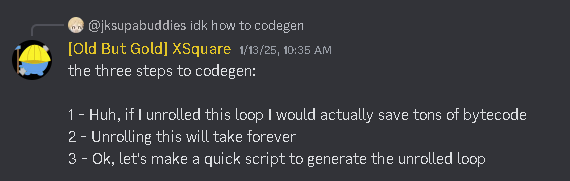
\includegraphics[scale=0.5]{images/unroll.png}
      \end{center}
      \item \textbf{Decision-making} - Your robots often have numerous goals they would like to fulfill. It may be tempting to tack on goal-types as you think of them, but this results in messy code that is difficult to modify. Additionally, it may be tempting to only store the current goal, but this results in your robots have very short-term memories (ie: they may forget their current task if they get initiated in a fight that overrides their current task). We propose the following framework:

    \medskip
      
      \textbf{Goal Priority Queue} - Each Goal contains the goal-type and the MapLocation where the goal is to be fulfilled. The priority for goals may depend on the game. For example, goal-types may be simple enough that they can be enumerated such that higher-numbered goals have a higher priority. However, if goal-types require more complicated priority, you can manually define them yourself.

    \medskip

      \textbf{Adding, Executing, and Stopping Goals} - Every goal type should have a shouldStartGoal, executeGoal, and shouldStopGoal methods. This modular design allows for easy modifications and additions to your goal framework.

    \medskip

      Note that this framework only applies to goal types that naturally interfere with one another. If a robot can fulfill multiple goal-types at once (ie: towers/archons attacking + spawning), those should each have their own priority queue.
      \item \textbf{Micro/Macro} - Micro and Macro refer to terminology from real-time-strategy games. Since Battlecode plays similarly to an RTS game, Micro and Macro are always applicable. Micro refers to fine-controlling singular robots, mostly to optimize robot-to-robot combat. Particularly, if a robot can fight another robot, there are certain movements/maneuvers robots can take to swing a fight in their favor. These include, but aren't limited to, weaving in and out of a robot's attack range, splitting robot groups to avoid area-of-affect attacks, kiting enemies, and pushing an engagement when a robot senses it has many allies. Macro refers to controlling army-level actions. These include, but aren't limited to, managing robot production, choosing when to expand, saving/spending your resources properly, and executing long-term strategic plans. While you can't explicitly plan a micro or macro strategy since they depend heavily on the game, it helps to have a framework for both. \href{https://github.com/IvanGeffner/BTC24/blob/master/MicroManager.java}{Here} is the infamous \textbf{XSquare} micro, a java file that has crushed many-a challenger. Nearly every other top team has benefited from copying the \textbf{XSquare} micro to some degree, and here's why:
      \begin{enumerate}
          \item \textbf{When to initiate micro (doMicro)} - The conditions to initiate micro are usually whether your robot can see enemy robots. However, this can be expanded to include cases such as having low hp and having memory of nearby enemies that may be out of vision.
          \item \textbf{The micro array (computeMicroArray)} - The micro array contains the heuristic information of all 9 movement options (moving to the 8 adjacent squares or staying still). This allows for easy updates to the heuristic information and comparing heuristic scores via loop unrolling.
          \item \textbf{Heuristic information (MicroInfo)} - The heuristic information stores all factors that make a tile appealing/dangerous to move to (ie: number of nearby enemies, distance to closest enemy, etc). Then, once all the heuristic information is calculated, the isBetterThan method can easily compare two MicroInfos. 
      \end{enumerate}
      Note that this micro only involves movement and not the actual attacking. This is because decision making for who and when to attack is usually straightforward (target the lowest hp enemy possible, attack whenever possible). Also note that \textbf{XSquare} micro could be completely rewritten with our Goal Priority Queue framework (we might do this next year).

      \medskip

      Macro is much more difficult to make a general framework for, since robot-spawning, resources, and high-level strategies vary drastically year-to-year. However, if you use ample communication, globally available info (such as map size), and the Goal Priority Framework, you should have no issue implementing the macro strategy you desire.

    
  \end{itemize}
  \item \textbf{Budget Your Time} - As mentioned previously, one of our big downfalls this year was spending a lot of time to perfect things that either don't need to be perfected. Battlecode is a short competition, and no one creates the perfect bot. Often the best tasks to do are the tasks with the best effort-to-result ratio. This frequently ends up being the simplest things, such as hard coding or using greedy algorithms.
  \item \textbf{Prioritize Economy} - Our workflow generally revolves around economy. The first thing we always do is plan how to get a strong economy as soon as possible. Battlecode games are often snow-bally, where any small resource lead can very quickly turn into a large advantages down the line. As a result, highly optimizing the beginning of games for resources is the best way to kickstart your team's snowball. Once you have done this, you can branch off into working on converting the economy into the win condition. Additionally, \textbf{Teh Devs} have historically shown favoritism to teams that prioritize economy-based gameplans (as opposed to rush/attack based gameplans) by making maps in the finals tournament larger and slower.
  \item \textbf{Learn from Others} - Watch replays, collaborate in the discord, talk with your teammates. Chances are you can learn something from every team out there, whether it is an insight or strategy they use, or some niche condition that breaks your bot. See where you are strong, see where you are weak, find out why you are weak, and figure out how to improve. Many top teams are very friendly, so don't be afraid to ask them what strategies they use on the Discord. Getting Battlecode clout is nearly as important as winning, so they will be happy to flex their superior Battlecode knowledge.
  \item \textbf{Stand on the Shoulders of Giants} - Similarly to the above, use every resource available to you. There are many past repositories that have been posted on the Discord. We view \textbf{XSquare} as the God of Battlecode. He has several years of his past bots posted \href{https://github.com/IvanGeffner}{here}, and has consistently been on top of the leaderboard. His micro, exploring, and pathfinding are all unmatched.
  \item \textbf{Test your code} - We have never bothered to write unit tests, but we realistically should. At minimum, run several games, closely analyzing whatever behavior you changed. Make custom maps, designed to expose your problems. Save old versions of your bot and compete against them. Run scrimmages against other teams. The more your code runs, the more problems you will find and fix. DO NOT upload untested bots right before important submission deadlines. At minimum, test against older versions of your code.
  \item \textbf{Use Git Effectively} - Git can be intimidating for first time users, but once you understand a few basic commands, it is really not too difficult. I cannot emphasize this enough, \textbf{learning command line git will save you and everyone you work with so much time and headache in the long run}. GUIs are good for the simple stuff, but you can break things in unimaginable ways by clicking buttons that you don't fully understand. Your team should have an agreed upon criteria for branching, commits, and reviews so that everyone is on the same page. Our recommended git workflow is below\footnote{We outline this in a lot of detail since we anticipate a lot of teams are using Battlecode to learn team programming, as we did in previous years.}:
  \begin{itemize}
    \item When you have a new feature you want to add, create a branch for it. This can be done as follows:
    \begin{verbatim}
      git fetch
      git checkout -b <branch-name> origin/main \end{verbatim}
    \verb|git fetch| will update your local reference to the remote repository (hosted on GitHub or elsewhere), and \verb|git checkout -b| will create a branch named \verb|<branch-name>| from the most up-to-date version of \verb|main| that is in \verb|origin| (the remote repository). Note that depending on how you have it configured, the main branch may be called \verb|master| instead.
    \item Make incremental progress on the code, and create a new commit every time you hit a ``checkpoint''. It is up to you to determine what that means, but I usually figure if I do a test run, its probably a good time for a commit. You can create a commit by doing the following:
    \begin{verbatim}
      git add <path-to-changes>
      git commit -m "<your-commit-message-here>" \end{verbatim}
    \verb|git add| will ``stage'' the changes at \verb|<path-to-changes>|, which is basically ``preparing them to be committed''. If you don't want to manually add each individual file, you can do \verb|git add .| to add all changes in the current directory, or \verb|git add <path-to-folder>/*| to add all changes in a folder. If you do either of these, you should run \verb|git status| after, and make sure the files listed as ``staged'' are the ones you intend to commit. If they are not, you can run \verb|git restore --staged| with a path to remove it from the staging area. \verb|git commit| creates a commit, and \verb|-m| adds the commit message.
    \item Once you have finished the feature you created the branch for, and have made all your commits, you are ready to merge back into \verb|main|. There are several ways of doing this, but our personal preference is using a rebase strategy, so we preserve a linear commit history without duplicate or merge commits. When you are ready to merge your code into main, do the following:
    \begin{verbatim}
      git fetch
      git rebase origin/main
      git push -u origin <branch-name> \end{verbatim}
    While the \verb|git fetch| and \verb|git rebase| steps are not fully necessary, they will save you from many problems in the future, and it is usually better to run them anyways. \verb|git rebase| moves the base of your branch to \verb|origin/main|, i.e., it takes the changes you made, and tries to re-apply them on the most up to date main. \textbf{Be sure to read the output of the rebase command}, as it may tell you there are conflicts. If so, open up your editor, most of them will have a conflict resolution tab, and fix the conflicts by choosing what to keep, change, or take out. This will only be necessary if you have multiple team members in different branches working on the same part of the code. Once you fix the conflicts, run \verb|git rebase --continue| and repeat if necessary. \verb|git push| sends your changes to the remote (GitHub), and \verb|-u origin <branch-name>| tells GitHub what the name of the branch should be. Make sure the \verb|<branch-name>| you give is the same as what you have locally. It shouldn't cause any problems, but it will certainly be confusing.
    \item Your branch should now have the latest version of \verb|main| with your new changes pushed on the end of it. To get these changes in \verb|main|, you should create a ``Pull Request'' on GitHub. You can do this either by following the link that shows up after you push, or going to GitHub and opening the ``Pull Requests'' tab. Add a name and description, and create the pull request. Your teammates should be able to view and comment on your changes. If you configure things correctly (and pay a monthly fee which we did not), you can pretty easily set up rules for GitHub to restrict merges until approval quotas have been met. When you are ready to merge the pull request, there is a big green button that shows up. \textbf{We recommend using the ``Rebase and merge''} strategy, so it preserves all the commits. This doesn't really matter most of the time, but it is annoying when you want to see what order you did things, or revert changes, and there are messy merge commits that make it hard to tell what was added.
    \item Make sure you run \verb|git checkout main| and \verb|git pull| to get the most up to date version of the code locally.
  \end{itemize}
  Again, this is just personal preference, and there are many other more detailed and thorough guides on similar strategies. What matters most is that you find something that your team agrees on and works for you. We have had similar success in the past with everyone battling it out on \verb|main| with no branches, so with a small enough team, no strategy can work as well.
\end{enumerate}

Obviously, there is more to Battlecode than just these points, but these are the biggest lessons we have learned and hope you find useful as well.

\subsection{Until Next Year\dots}

We hope you found this writeup useful, entertaining, inspiring, or positive in some other way. We have really enjoyed the ups and downs of Battlecode every year, and will definitely continue competing even after our eligibility is gone. Next year is definitely the last year for Justin, and probably the last year for Andrew, and we are really hoping to make something special happen. After that, we will make it our mission to win a sprint tournament, we need that discord role.

\begin{figure}[H]
  \centering
  
\includegraphics[scale=0.5]{images/caterpillow.png}
  \caption{Subscribe to \textbf{caterpillow}}
\end{figure}

As always, thank you to \textbf{Teh Devs} for creating and running such a fantastic competition this year and every previous year we have competed. Huge thank you to all the other teams we mentioned previously in this document, particularly \textbf{XSquare} for his 10 year commitment to dominating the Battlecode leaderboard and open sourcing his code every year. Congrats to the winners, \textbf{Just Woke Up}, after an insane set of rematches against \textbf{Confused}, an impressive individual competitor, and \textbf{podemice} with the upset of the year in US Qualifiers.

\medskip

We are incredibly excited for next year, and hope to continue our trend of improvement.
